% !TeX encoding = UTF-8
% !TeX spellcheck = es_ES
% !TeX root = ../../main.tex


\epigraph{Los hombres no crecen, solo cambian el precio y tamaño de sus juguetes}{Cita anonima en Internet}

\begin{abstract}
Hay varias formas de jugar con una maqueta de tren, en este capitulo se revisaran algunas de las más comunes
\end{abstract}

\section{Introducción}
La mayoría de aficionados, como el autor, empiezan con una caja de iniciación. Montando un óvalo y dando vueltas, lo que sinceramente tras unas cuantas, es un poco más divertido que ver secarse la pintura, aunque no mucho más.

En este momento, el aficionado común, es cuando decide montarse su propia maqueta. Busca el espacio más grande que dispone y en definitiva, siendo su primera maqueta, hace una revisión del óvalo. Más grande, con más vías y desvíos, pero al final se tratará de lo mismo. Dar vueltas.

Lo cierto es que con esta maqueta habrá puesto alguna estación con apartadero, o una playa de vías, o algo con lo que maniobrar. Con esta experiencia acabará haciendo una maqueta nueva que se vaya ajustando a una forma de jugar.

\begin{figure}[h]
	\centering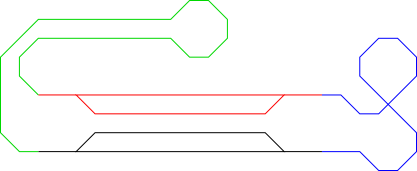
\includegraphics[]{chapters/01_jugar/maqueta.png}
	\caption{Maqueta un poco más compleja (pero un ovalo al fin y acabo)}
	\label{fig:maqueta}
\end{figure}

A este aficionado quizás le guste más simular las operaciones de una línea, o resolver puzzles “time-saver ” o … Al final hay tantas formas de jugar como aficionados. Y la maqueta personal se deberá hacer con forme se piense que se va a jugar con ella.

Este es un proceso que se debe pasar y existen errores que se deben cometer si se quiere disfrutar al máximo. Aunque es posible tomar algún atajo, siempre y cuando al final sepa como va a jugar. Si algún amigo tiene ya una maqueta o siendo socio de un club, tendrá a su disposición unas primeras maquetas con las que aprender cómo jugar.

Otro atajo es leer foros y artículos de revistas. Entorno al 2019/06/03 en forotrenes publicaron unos pdfs hablando sobre una serie de artículos explicando cómo planificaron una maqueta según una explotación realista. Y la conclusión que podemos obtener es la misma. Pensar antes como jugar y el contexto (de la línea imaginada) y luego diseñar la maqueta.

Bueno, teniendo claro que antes de diseñar una maqueta (e incluso antes de buscar el espacio) tenemos que saber como jugar, queremos saber que formas de jugar hay.

\section{Estado del arte}
Unos grupos iniciales de como jugar serán y de los que es fácil encontrar información:

\begin{itemize}
	\item Time-Saver o Puzzles
	\item Cartas o Americano
	\item Explotación o Europeo
	\item Exhibición
\end{itemize}
Así mismo hay otras formas que no se dicen expresamente, pero que se nombran o se intuyen.
\begin{itemize}
	\item Libre
	\item Otras formas Regladas
\end{itemize}
\subsection{Time Saver o Puzzles}
Son maquetas pequeñas y, por norma general, lineales abiertas. Una vía recta recorre toda la longitud y representa la línea principal, de la cual sale una zona de maniobras.
\begin{figure}[h]
	\centering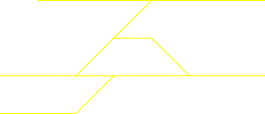
\includegraphics[]{chapters/01_jugar/path4865.png}
	\caption{Ejemplo TimeSaver}
	\label{fig:timesaver} % Unique label used for referencing the figure in-text
	%\addcontentsline{toc}{figure}{Figure \ref{fig:placeholder}} % Uncomment to add the figure to the table of contents
\end{figure}

En la maqueta se colocan una máquina (tractor de maniobras ) y varios vagones, siguiendo una disposición inicial. Además se tiene un plano con la situación final.

El juego se trata que moviendo el tractor, enganchado y desenganchado vagones, cambiando agujas y demás hasta se llegue a la situación final.

La reglas son sencillas, los trenes van por la vía y no se puede usar la mano (salvo desenganches y descarrilamientos). Se puede jugar en solitario, o compitiendo contra otros, en dicho caso, gana quien tarde menos (en tiempo o en pasos).

\subsection{Cartas o Sistema Americano}
Se llama Sistema Americano porque es el preferido en EEUU, se trata de tener todo el material en la maqueta y que todo el mismo se mueva.

A cada vagón se le asigna una tarjeta. En la cual se le asignan 4 destinos y se trata que todos los vagones recorran sus cuatro destinos. El último destino se considera su base y debe ser el punto de inicio.

Para facilitar el juego en cada destino se pone un cajetín con los vagones que tiene. Las cartas son pequeñas y los destinos se escriben de tal forma que girándola carta quede visible en el cajetín el próximo destino del vagón. El operador de dicho destino tiene que hacer una nueva composición y enviar el nuevo tren por una línea que acerque cada vagón a su siguiente destino.

\begin{figure}[h]
	\centering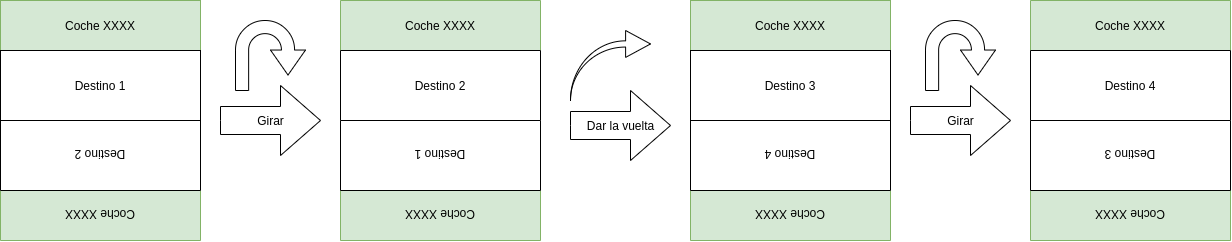
\includegraphics[width=\textwidth]{chapters/01_jugar/HowToPlay-cartas.png}
	\caption{Ejemplo de Carta}
	\label{fig:cartas} % Unique label used for referencing the figure in-text
	%\addcontentsline{toc}{figure}{Figure \ref{fig:placeholder}} % Uncomment to add the figure to the table of contents
\end{figure}

Es necesario tener una maqueta grande, donde incluir múltiples destinos. Y en esos destinos tener una zona para maniobrar donde crear nuevas composiciones. En estados unidos, es mas usual vivir en unifamiliares y tener un sótano más grande donde poner la maqueta.

También se pueden jugar varios encargándose cada uno de una zona (varios destinos)

\subsection{Explotación Real o Sistema Europeo}
Como el anterior, es el preferido en Europa y por eso se llama sistema Europeo. En este caso la maqueta se diseña simulando una línea “real”. El jugador o maquetista sera el dueño de una compañía ficticia. O al menos el responsable de gestionar los trenes para dicha compañía.

Se parte de un contexto o motivo que justifique la misma, sus elementos y su paisaje. Por ejemplo una ciudad pesquera con su estación de termino con comunicaciones a la capital y un pueblo intermedio. En este ejemplo la industria pesquera recibe los pescados del pueblo y los enviá a la capital. La gente de la capital utiliza el pueblo como destino turístico. 

Con estos datos se planificaran las estaciones, dos términos y un apeadero en medio. Así mismo se incluirán las naves de mantenimiento, bases, playas de vías, etc …. Para alargar un poco el juego, se incluirá un ovalo que permita alargar el recorrido. En general es una linea punto a punto, como sucede en la realidad. Si bien se añadido un ovalo en pos de la jugabilidad.

\begin{figure}[h]
	\centering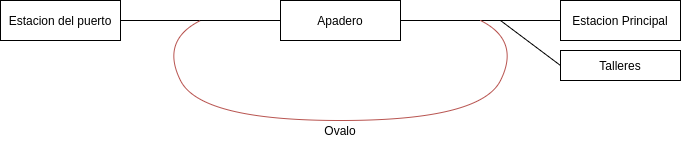
\includegraphics[width=\textwidth]{chapters/01_jugar/HowToPlay-EU.png}
	\caption{Ejemplo de explotación}
	\label{fig:explotacion} % Unique label used for referencing the figure in-text
	%\addcontentsline{toc}{figure}{Figure \ref{fig:placeholder}} % Uncomment to add the figure to the table of contents
\end{figure}

Para jugar con esta maqueta sera conveniente así mismo pensar o definir las reglas de operaciones:

\begin{itemize}
	\item Prioridades de trenes (Alta Velocidad, Pasajeros, Mercancías perecederas, …)
\item Reglas de paso (los trenes mercantes pasan por vías sin anden, la vía no desviada no tiene anden, se reserva para pasos sin parada,…)
\item Reglas de dirección (en doble vía por la derecha, los que van hacia el pueblo pesquero paran en vías pares,…)
\item …
\end{itemize}
También se tendrá que pensar en los trenes regulares (Expresos nocturnos, regionales mercancías, …) como se nombran e identifican. Con esto se podrá crear una tabla de horarios para cada estación.

En ultimo lugar, pero no por ello menos importante, unas reglas para la maqueta o de compresión de la realidad serán necesarias. En el ejemplo, se define que para ir del pueblo a la capital hay que dar 5 vueltas al ovalo, y el apeadero esta en la vuelta 3. Otra regla de compresión, es el reloj acelerado (1 hora en la realidad son 3 en el juego, por ejemplo) o que tal vagón puede cargar X pasajeros o Y toneladas y, por lo tanto, necesita un tiempo definido para carga y descarga.

El objetivo es siempre el mismo: optimizar el uso del material siendo capaces de cumplir la tabla de horarios que se haya definido. Pero se puede complicar todo lo que se quiera (mantenimiento periódico, costes de carburante,…)

Este sistema se prefiere en Europa ya que poca gente tiene un gran espacio donde montar su maqueta y es muy fácil ajustarlo al espacio disponible:

Si tenemos poco espacio podemos diseñar una estación que ocupe lo máximo posible y preocuparlos solamente por gestionar los trenes que entran y salen de ella. Para que el juego sea interesante debe ser una estación principal donde haya que entrar o sacar un tren cada poco y ademas montar y desmontar composiciones, fuera de la estación puede ser una playa de vías con varias composiciones preparadas o montarlas a mano.

Si tenemos mucho espacio podemos hacer una linea completa con varias estaciones, industrias,…

Nos ayudara mucho hacernos un cronograma de donde va estar cada tren en cada momento.

\subsection{Exhibición}

\section{¿Que tenemos ademas?}

\subsection{Libre}
Obviamente lo anterior son las categorías que he ido viendo por internet, luego cada uno se pude organizar como quiera.

En el juego libre movemos nuestros trenes sin una razón ni reglas concretas. Ahora muevo el talgo, luego el mixto, paro este aquí,….

En esta categoría incluyó la exhibición. Y es mover los trenes con el objetivo de que alguien los vea. No solo el propio tren, sino también la maqueta.

Ademas en este apartado podemos hablar de rodaje técnico, o mover las piezas para que la mecánica no se oxide…Paragraph

Esta categoría agrupa todas las formas de jugar que moveremos los trenes sin un sistema de reglas o sin objetivo claro.

\subsection{Otras Formas Regladas}
Aquí agrupo otras formas, no tan extendidas de jugar, pero regladas. Al final cada uno tiene su maqueta y juega como quiere.

Por ejemplo en las exposiciones y encuentro de modelos, se suele hacer una tabla de horarios y unas composiciones y se trata de que cada modulista se encarga de una zona (varios módulos) y se debe cumplir el horario dicho. Amen de otras reglas que dicte el organizador.

Si vamos a un encuentro de módulos como visitantes veremos a un grupo de “amigos” que se mandan trenes de uno a otro, siempre atentos a los trenes y a los controles. Si queremos preguntar algo de la maqueta, nos dirigiremos, o nos responderá alguien que no este a los mandos en ese momento.

Por otra parte si vamos a una exposición, las maquetas las habra hecho una sola persona, o un grupo reducido de personas (en general). Habra un tren dando vueltas, para que se vea como queda. Pero básicamente el tren andará solo, no se parara en las estaciones y el dueño estará vigilando que los visitantes no metan las zarpas (digo las manos) en medio de la maqueta y resolviendo dudas y preguntas de los visitantes.

\section{Resultados o Datos de interés}(Opcional) 
Si es un experimento incluir los datos o resultados obtenidos, sin valorar ni judgar. Es buen lugar para incluir otros detalles encontrados durante la escritura, búsqueda de información,....
\section{Discusión}
Este el punto para valorar los resultados y dar opiniones.
\section{Conclusiones}
Resumir y agrupar los resultados obtenidos
\section{Próximos pasos}
Escribir aquí un breve texto de lo que se hablara en otros capítulos (y que tenga referencia con este), o cosas que se dejan para realizar en un futuro fuera de este PDF.
\section{Bibliografía y Referencias}
\printbibliography[heading=subbibliography]